\documentclass[11pt,UTF8]{ctexart}
\usepackage{titling}
\usepackage{enumerate}
\usepackage{amsmath,amssymb,amsfonts}
\usepackage{listings}
\usepackage{comment}
\usepackage{forest}
\usepackage{bm}
\usepackage{float}
\usepackage{graphicx}
\usepackage{multicol,multirow}
\usepackage{bigstrut}
\usepackage[unicode=true,%本行非常重要 支持中文目录hyperref CJKbookmarks对二级目录没用
	colorlinks,
	linkcolor=black,
	anchorcolor=black,
	citecolor=black,
	CJKbookmarks=false]{hyperref}
\usepackage{xcolor}
\usepackage{geometry}
\geometry{top=20mm,bottom=20mm,left=20mm,right=20mm}
\pagestyle{plain}%删除页眉
\CTEXsetup[format={\Large\bfseries}]{section}

\lstset{basicstyle=\small}

\def\toprule{\hline}
\def\midrule{\hline}
\def\bottomrule{\hline}
\newcommand{\ol}[1]{\mathop{\overline{#1}}}%\mathop important!!!

\setlength{\droptitle}{-50pt}%减少标题与页眉距离

\title{数电期末大作业实验报告}
\author{17341015\quad数据科学与计算机学院\\计科一班\quad陈鸿峥}
\date{}

\begin{document}
\maketitle
\vspace{-50pt}%减少标题与正文距离
\lstset{language=C++,escapechar=`}

\section{内容一}
\subsection{实验目的}
使用Proteus和Basys3实验板实现具有分、秒计时的计数器

\subsection{实验原理}
\begin{enumerate}
    \item 通过两个十进制计数器74LS160级联,实现60进制计数,具体实施方法如下
    \begin{itemize}
        \item 第一个74LS160的进位端RCO与第二个74LS160的两个使能端ENP、ENT相连,代表计数到10,进位时,第二个计数器才开始工作
        \item 第一个74LS160的其余端口(使能端ENP、使能端ENT、置数信号端$\overline{LOAD}$、清零端$\overline{MR}$)均连接高电平,置数端D0、D1、D2、D3均不连接
        \item 第二个74LS160的清零端连接高电平,置数端D0、D1、D2、D3均连接低电平,代表从0000开始计数
        \item 第一个74LS160的输出端Q3、Q0、第二个74LS160的输出端Q2、Q0与一个与非门连接后连入第二个74LS160的置数信号端,代表计数至十进制的59时,传递信号给第二个74LS160准备重新从0000开始计数
        \item 所有74LS160接同一个时钟(1Hz)
    \end{itemize}
    \item 将两个上述的60进制计数器再进行级联,即可分别实现分和秒的计数。注意第三个74LS160的使能端通过上一个74LS160的输出控制,即59时才准备运作。第四个74LS160是在``59:59''时才清零计数,故还需与第一个60进制计数器连接一个与门进行判断
    \item 4个74LS160的输出端Q0、Q1、Q2、Q3分别与4个74LS48译码器的A、B、C、D端口相连,其$\ol{BI/RBO}$、$\ol{RBI}$、$\ol{LT}$端全部连接高电平
    \item 由于是通过扫描显示数码(时钟10kHz),故用4个四选一选择器74LS153来选择对应7段数码管ABCDEFG的输出,其使能端$\ol{E}$均接低电平
    \item 再用1个四选一选择器74LS139选择对应数码段的选通
\end{enumerate}

\subsection{Proteus仿真}
\begin{figure}[H]
    \centering
    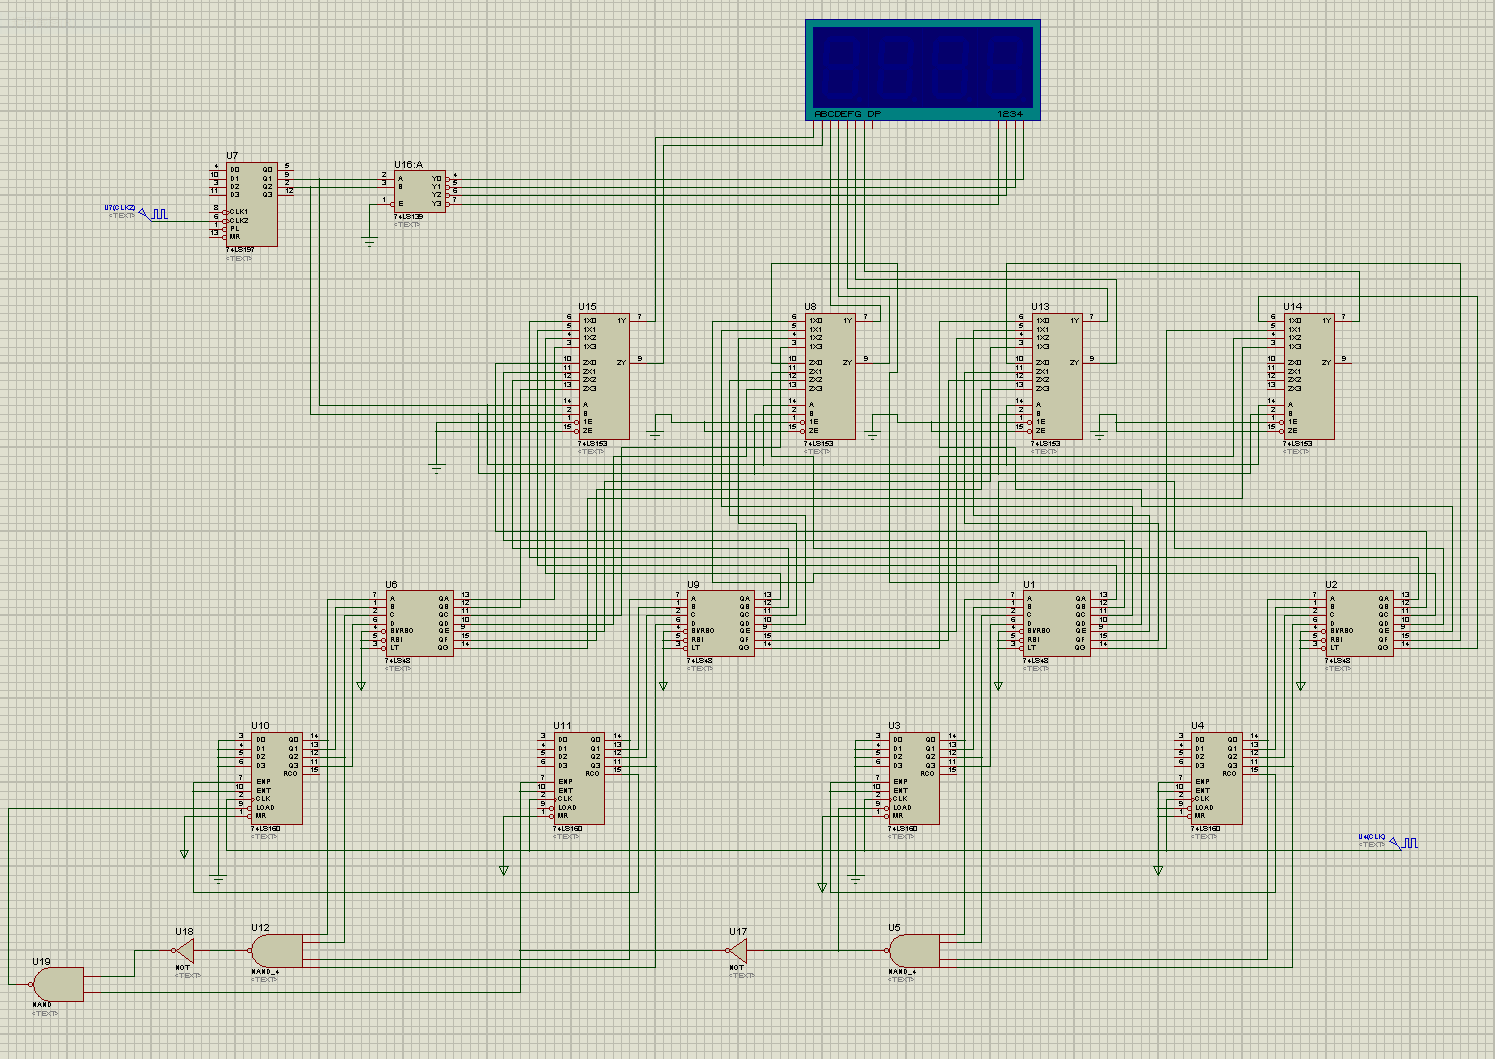
\includegraphics[width=\linewidth]{fig/Counter_1.PNG}
\end{figure}

\subsection{Basys3实现原理}
\begin{enumerate}
    \item 先将$10^9$Hz的时钟进行分频,变为$1$Hz和$10^4$Hz,$1$Hz用于计数,$10$kHz用于显示
    \item 分别用四个计数器,表示10s、1min、10min以及99min的计数,也即四位数码管上显示的内容
    \item 注意触发器状态的转换应考虑上一状态,因存在延时,同时用下降沿negedge触发,解决初始值问题
\end{enumerate}

\subsection{Basys3电路实现}
\par Verilog程序如下,计数器及分频部分
\begin{lstlisting}[language=Verilog,basicstyle=\tiny]
module Counter(
    input clr, // clear, say reset
    input wire clk, // clock
    input wire fb, // front or back
    output [6:0] seg,
    output reg [3:0] an
    );
    
    // display 10kHz
    reg [16:0] count_dis; // 26 bits to store count: 2^17 > 10^5
    reg clk_dis;
    always @ (posedge clk or posedge clr)
    begin
        if (clr == 1) // reset
        begin
            clk_dis <= 0;
            count_dis <= 0;
        end
        else if (count_dis == 50_000 - 1) // return 0
        begin
            clk_dis <= ~clk_dis;
            count_dis <= 0;
        end
        else
        begin
            clk_dis <= clk_dis;
            count_dis <= count_dis + 1;
        end
    end

    reg [1:0] out;
    always @ (posedge clk_dis or posedge clr)
    begin
        if (clr == 1 || out == 4)
            out <= 0;
        else
            out <= out + 1;
    end

    // time counter + frequency divisor (flip-flop)
    // 1s
    localparam MAX_COUNT_FEQ = 50_000_000; // 0.5s
    reg [25:0] count_ns; // 26 bits to store count: 2^26 > 10^5
    reg clk_sec;
    always @ (posedge clk or posedge clr)
    begin
        if (clr == 1) // reset
        begin
            clk_sec <= 0;
            count_ns <= 0;
        end
        else if (count_ns == MAX_COUNT_FEQ - 1) // return 0
        begin
            clk_sec <= ~clk_sec;
            count_ns <= 0;
        end
        else
        begin
            clk_sec <= clk_sec;
            count_ns <= count_ns + 1;
        end
    end

    // 10s time counter
    reg [3:0] count_sec_1;
    reg clk_10s;
    always @ (posedge clk_sec or posedge clr)
    begin
        if (clr == 1)
        begin
            clk_10s <= 0;
            count_sec_1 <= 0;
        end
        else
        begin
            if (count_sec_1 == 4) // frequency divisior
                clk_10s <= ~clk_10s;
            if (count_sec_1 == 9) // next stage
            begin
                count_sec_1 <= 0;
                clk_10s <= ~clk_10s;
            end
            else
                count_sec_1 <= count_sec_1 + 1;
        end
    end

    // 1min
    reg [3:0] count_sec_2;
    reg clk_min;
    always @ (negedge clk_10s or posedge clr)
    begin
        if (clr == 1)
        begin
            count_sec_2 <= 0;
            clk_min <= 0;
        end
        else
        begin
            if (count_sec_2 == 2)
                clk_min <= ~clk_min;
            if (count_sec_2 == 5)
            begin
                count_sec_2 <= 0;
                clk_min <= ~clk_min;
            end
            else
                count_sec_2 <= count_sec_2 + 1;
        end
    end

    // 10min
    reg [3:0] count_min_1;
    reg clk_10m;
    always @ (negedge clk_min or posedge clr)
    begin
        if (clr == 1)
        begin
            count_min_1 <= 0;
            clk_10m <= 0;
        end
        else
        begin
            if (count_min_1 == 4)
                clk_10m <= ~clk_10m;
            if (count_min_1 == 9)
            begin
                count_min_1 <= 0;
                clk_10m <= ~clk_10m;
            end
            else
                count_min_1 <= count_min_1 + 1;
        end
    end

    // 99min
    reg [3:0] count_min_2;
    always @ (negedge clk_10m or posedge clr)
    begin
        if (clr == 1)
            count_min_2 <= 0;
        else if (count_min_2 == 9)
                count_min_2 <= 0;
            else
                count_min_2 <= count_min_2 + 1;
    end

    display disp1 (.dis(out),
                   .count_sec_1(count_sec_1),
                   .count_sec_2(count_sec_2),
                   .count_min_1(count_min_1),
                   .count_min_2(count_min_2),
                   .seven_seg(seg));

    always @ (out)
        case (out)
            0: an = 4'b1110;
            1: an = 4'b1101;
            2: an = 4'b1011;
            3: an = 4'b0111;
        endcase

endmodule
\end{lstlisting}
\par 七段数码管显示部分
\begin{lstlisting}[language=Verilog,basicstyle=\tiny]
module display (
    input [1:0] dis,
    input [3:0] count_sec_1, // 2^4 > 10
    input [3:0] count_sec_2, // 2^3 > 6 still use 4 bits
    input [3:0] count_min_1,
    input [3:0] count_min_2,
    output reg [6:0] seven_seg
    );

    // seven segments
    parameter _0    = 7'b000_0001;
    parameter _1    = 7'b100_1111;
    parameter _2    = 7'b001_0010;
    parameter _3    = 7'b000_0110;
    parameter _4    = 7'b100_1100;
    parameter _5    = 7'b010_0100;
    parameter _6    = 7'b010_0000;
    parameter _7    = 7'b000_1111;
    parameter _8    = 7'b000_0000;
    parameter _9    = 7'b000_0100;

    always @ (dis)
    case (dis)
        0: // units (second)
        case (count_sec_1)
            0: seven_seg = _0;
            1: seven_seg = _1;
            2: seven_seg = _2;
            3: seven_seg = _3;
            4: seven_seg = _4;
            5: seven_seg = _5;
            6: seven_seg = _6;
            7: seven_seg = _7;
            8: seven_seg = _8;
            9: seven_seg = _9;
        endcase // count
        1: // tens (second)
        case (count_sec_2)
            0: seven_seg = _0;
            1: seven_seg = _1;
            2: seven_seg = _2;
            3: seven_seg = _3;
            4: seven_seg = _4;
            5: seven_seg = _5;
            6: seven_seg = _6;
            7: seven_seg = _7;
            8: seven_seg = _8;
            9: seven_seg = _9;
        endcase // count
        2: // units (minute)
        case (count_min_1)
            0: seven_seg = _0;
            1: seven_seg = _1;
            2: seven_seg = _2;
            3: seven_seg = _3;
            4: seven_seg = _4;
            5: seven_seg = _5;
            6: seven_seg = _6;
            7: seven_seg = _7;
            8: seven_seg = _8;
            9: seven_seg = _9;
        endcase // count
        3: // tens (minute)
        case (count_min_2)
            0: seven_seg = _0;
            1: seven_seg = _1;
            2: seven_seg = _2;
            3: seven_seg = _3;
            4: seven_seg = _4;
            5: seven_seg = _5;
            6: seven_seg = _6;
            7: seven_seg = _7;
            8: seven_seg = _8;
            9: seven_seg = _9;
        endcase // count
    endcase // dis

endmodule
\end{lstlisting}
\par 限制文件如下
\begin{lstlisting}[language=Verilog,basicstyle=\tiny]
set_property PACKAGE_PIN W4 [get_ports {an[3]}]
set_property PACKAGE_PIN V4 [get_ports {an[2]}]
set_property PACKAGE_PIN U4 [get_ports {an[1]}]
set_property PACKAGE_PIN U2 [get_ports {an[0]}]
set_property PACKAGE_PIN W7 [get_ports {seg[6]}]
set_property PACKAGE_PIN W6 [get_ports {seg[5]}]
set_property PACKAGE_PIN U8 [get_ports {seg[4]}]
set_property PACKAGE_PIN V8 [get_ports {seg[3]}]
set_property PACKAGE_PIN U5 [get_ports {seg[2]}]
set_property PACKAGE_PIN V5 [get_ports {seg[1]}]
set_property PACKAGE_PIN U7 [get_ports {seg[0]}]

set_property PACKAGE_PIN W5 [get_ports clk]
set_property IOSTANDARD LVCMOS33 [get_ports {an[3]}]
set_property IOSTANDARD LVCMOS33 [get_ports {an[2]}]
set_property IOSTANDARD LVCMOS33 [get_ports {an[1]}]
set_property IOSTANDARD LVCMOS33 [get_ports {an[0]}]
set_property IOSTANDARD LVCMOS33 [get_ports {seg[6]}]
set_property IOSTANDARD LVCMOS33 [get_ports {seg[5]}]
set_property IOSTANDARD LVCMOS33 [get_ports {seg[4]}]
set_property IOSTANDARD LVCMOS33 [get_ports {seg[3]}]
set_property IOSTANDARD LVCMOS33 [get_ports {seg[2]}]
set_property IOSTANDARD LVCMOS33 [get_ports {seg[1]}]
set_property IOSTANDARD LVCMOS33 [get_ports {seg[0]}]
set_property IOSTANDARD LVCMOS33 [get_ports clk]

set_property PACKAGE_PIN V17 [get_ports clr]
set_property IOSTANDARD LVCMOS33 [get_ports clr]
\end{lstlisting}
\par 最终结果图如下
\begin{figure}[H]
    \centering
    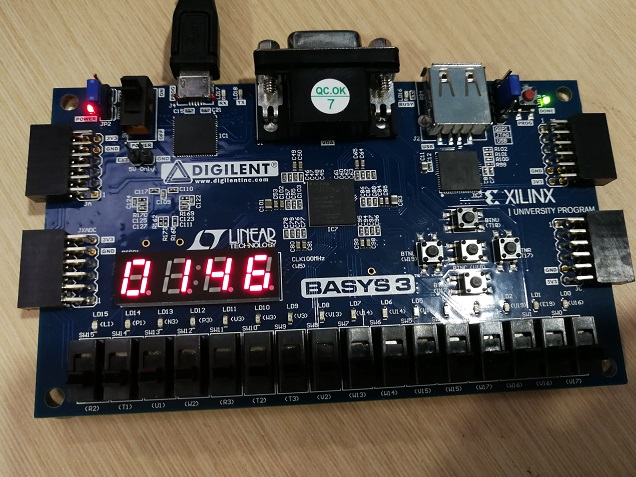
\includegraphics[width=\linewidth]{fig/board.jpg}
\end{figure}
\par 其中,最右的拨码开关V17用于清零


\section{内容二}
\subsection{实验目的}
在内容一Proteus设计的基础上给计时器添加调整当前时间的功能,即添加进入调整计时模式(MOD)按键和分/秒循环加一(ADJ)按键

\subsection{实验原理}
\begin{enumerate}
    \item 基础电路同内容一
    \item MOD按键相当于用来控制CLK,若为0,则CLK为连续脉冲,时钟自己走;若为1,则为孤立脉冲,时钟处在调整态
    \item 处在调整模式下,ADJ每次变为高电平,相当于给CLK一个孤立脉冲,则只需添加一个二选一选择器即可实现要求
\end{enumerate}

\subsection{Proteus仿真}
\begin{figure}[H]
    \centering
    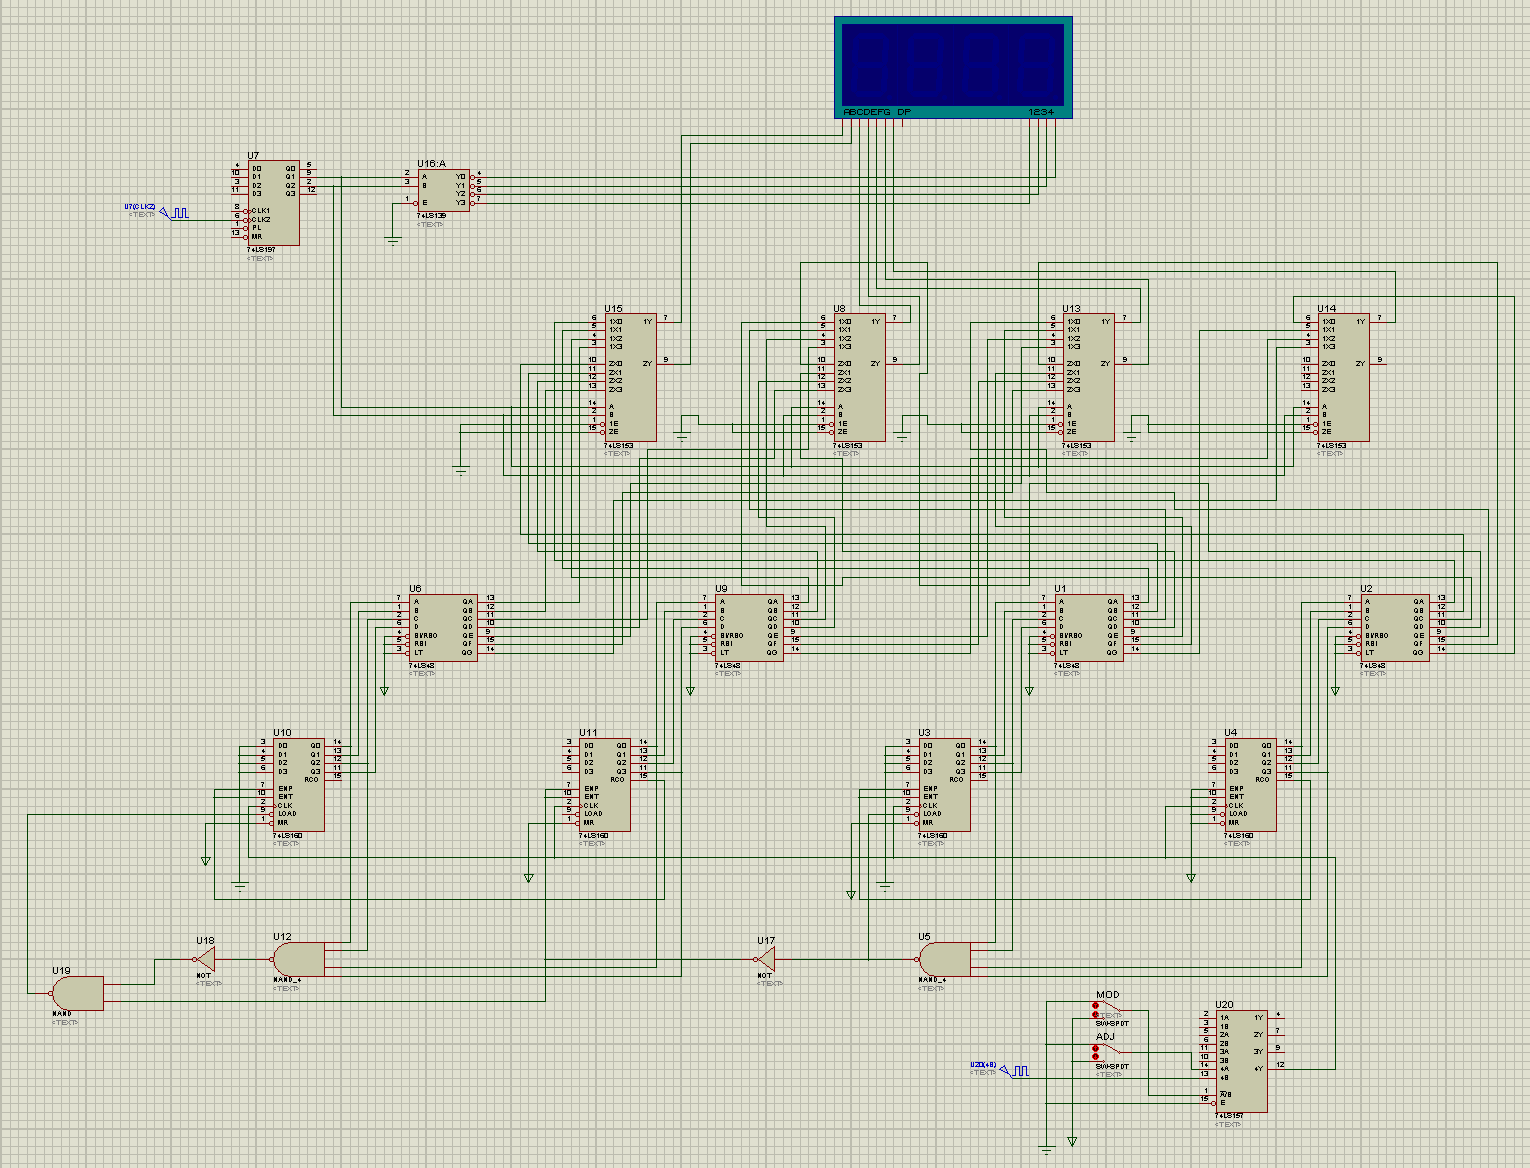
\includegraphics[width=\linewidth]{fig/Counter_2.PNG}
\end{figure}


\section{内容三}
\subsection{实验目的}
使用Proteus实现具有年、月、日、时、分、秒计时的计时器,计时结果显示在7段数码管上,要求年、月、日、时、分、秒均可调节

\subsection{实验原理}
\par 本实验原理同前两个内容,但是需要考虑的细节相当多
\begin{enumerate}
    \item 由于有MOD模式,故将CLK与MOD模式下的单步脉冲分开,即在正常模式下,所有计数器都接相同的时钟,在MOD模式下,则分别对应不同按钮,按下去即给出单步脉冲
    \item 使能端与时钟均需进行判断,故用74LS157进行选择
    \item 由于在调整过程中,可能出现高位先清零的情况(如23:20:00继续调节hour),故需要在置数端加一个判断,即处在MOD模式下才允许高位先清零
    \item 进位的问题,由于存在延时,故同样需要加入判断,调整模式下,上一RCO为1则下一使能端时钟均为1
    \item 由于74LS160不提供预先设数功能,故要自行设置一个预置端(PRE),一开始将2018年1月1日传入
    \item 月份大小的问题,实际上只有28、29、30、31四种情况,分别编号为00、01、10、11,同时用16选1选择器74150选择1月到12月这十二种状态. 注意其实只有2月是0开头,故只用一个74150对第二位数字进行选择即可实现大小月
    \item 闰年判断需要做一个模4计数器,但由于模4的特性,即只需看最后两位,故通过观察寻找规律我们得知:当十位为偶数时,个位只能为0或4或8;当十位为奇数时,个位只能为2或6. 故通过74154元件4线-816线选择器,可以将被4整除的年份选取出来. 同样的道理对百位和千位进行操作,可以实现模400. 至于模100,只需检测第二个进位端是否有进位即可. 再通过逻辑门判断即可选出闰年,即模4余0且模100不为0或模400余0的年份.
\end{enumerate}

\subsection{Proteus仿真}
\par 总体电路图如下
\begin{figure}[H]
    \centering
    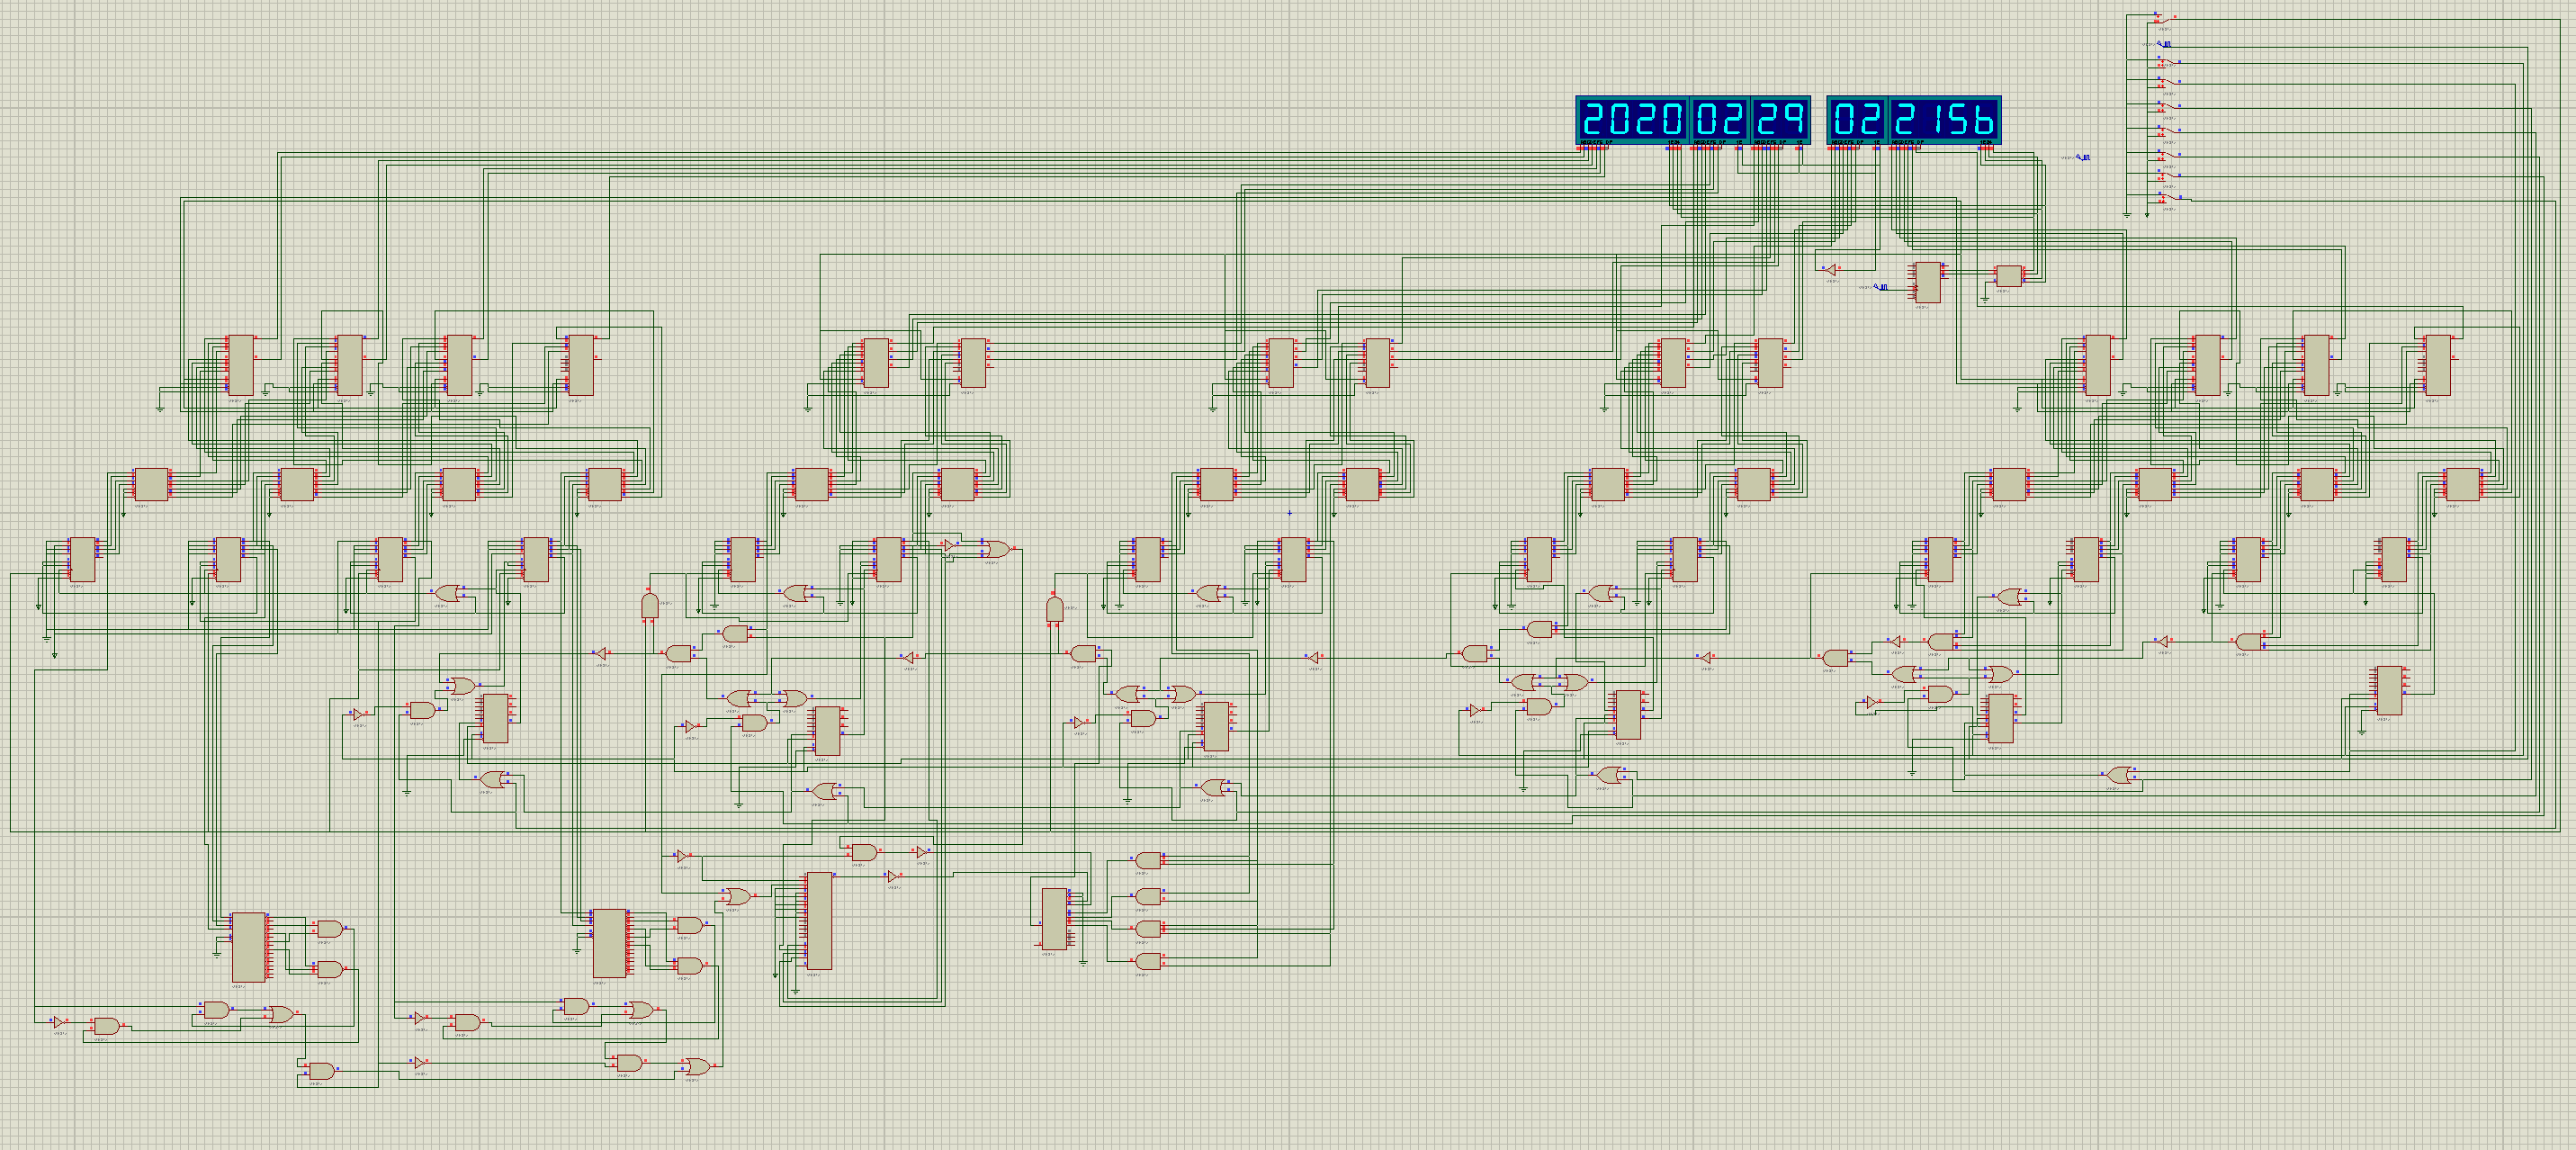
\includegraphics[width=\linewidth]{fig/Counter_4.PNG}
\end{figure}
\par 时间部分电路图如下
\begin{figure}[H]
    \centering
    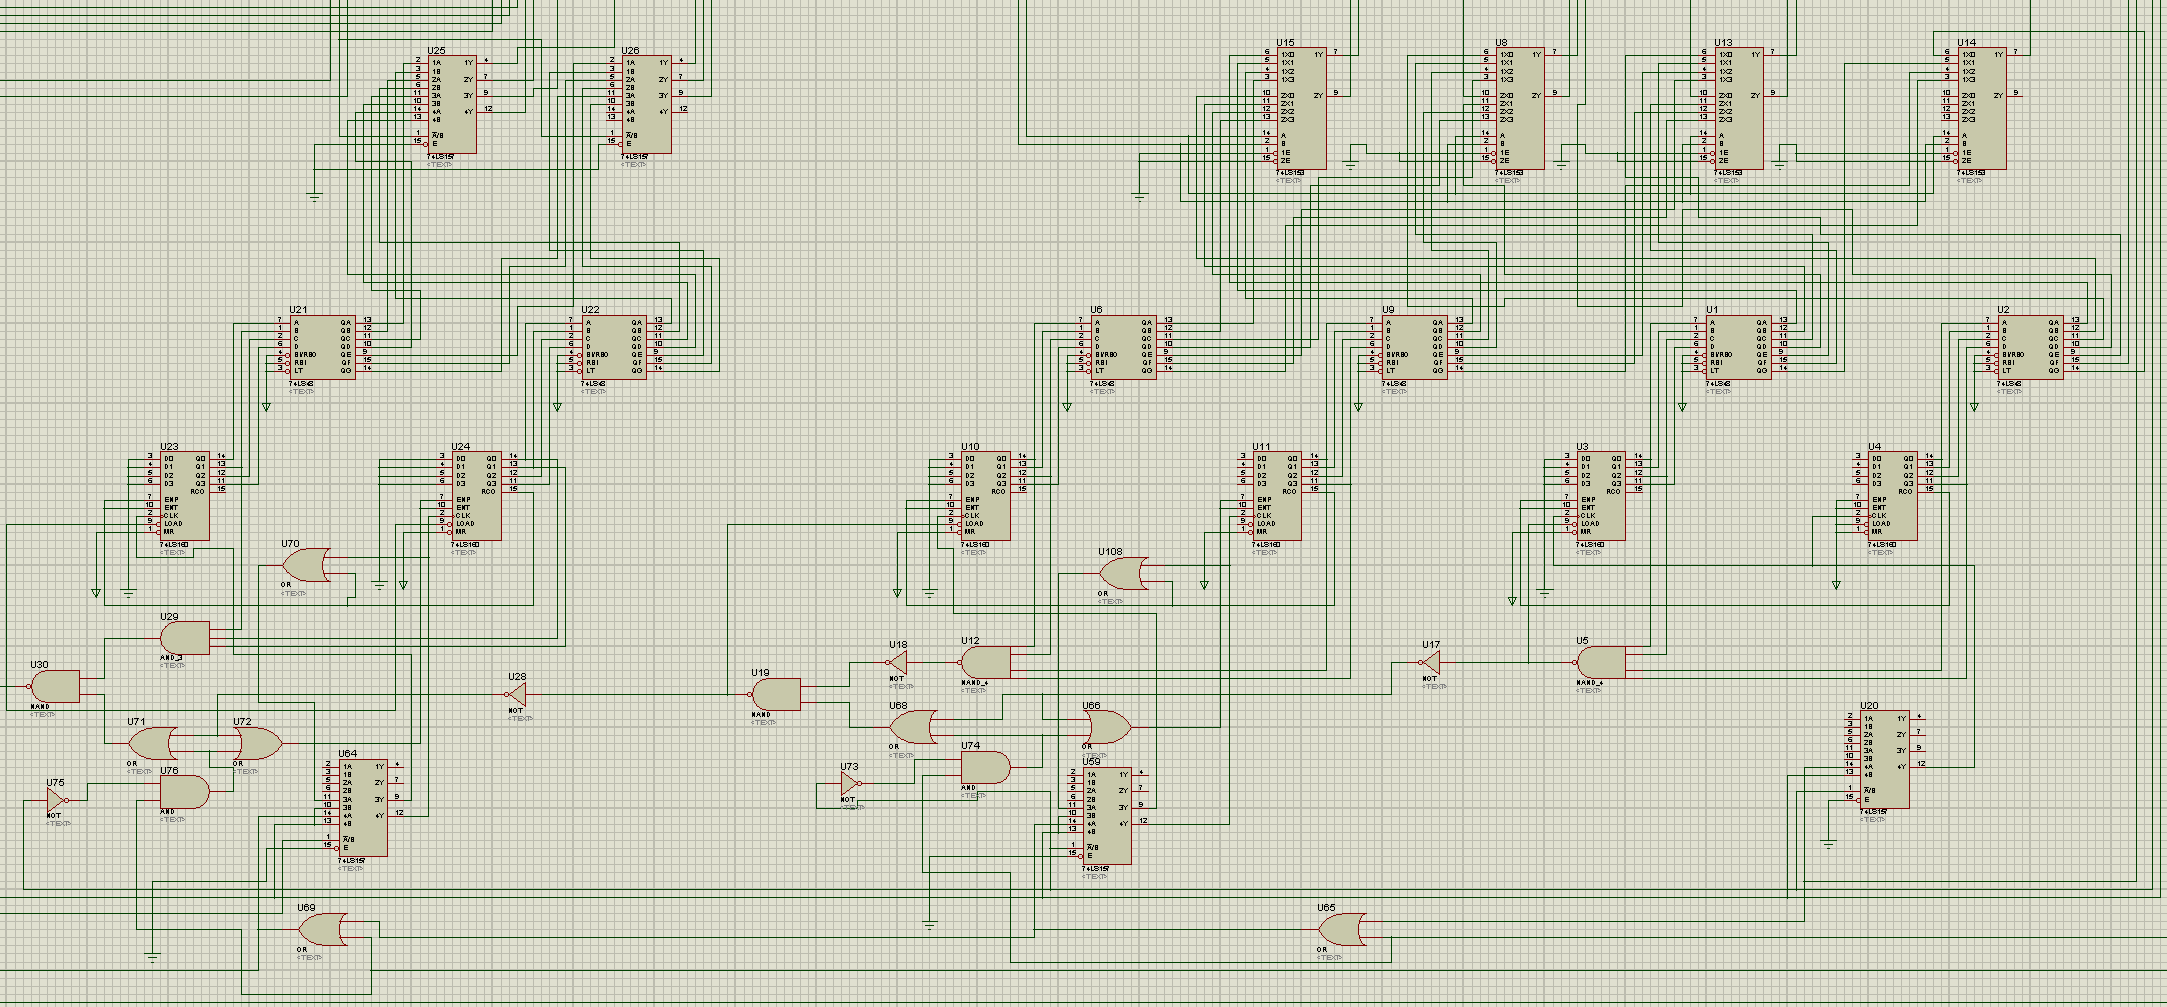
\includegraphics[width=\linewidth]{fig/Counter_3_time.PNG}
\end{figure}
\par 日期部分电路图如下
\begin{figure}[H]
    \centering
    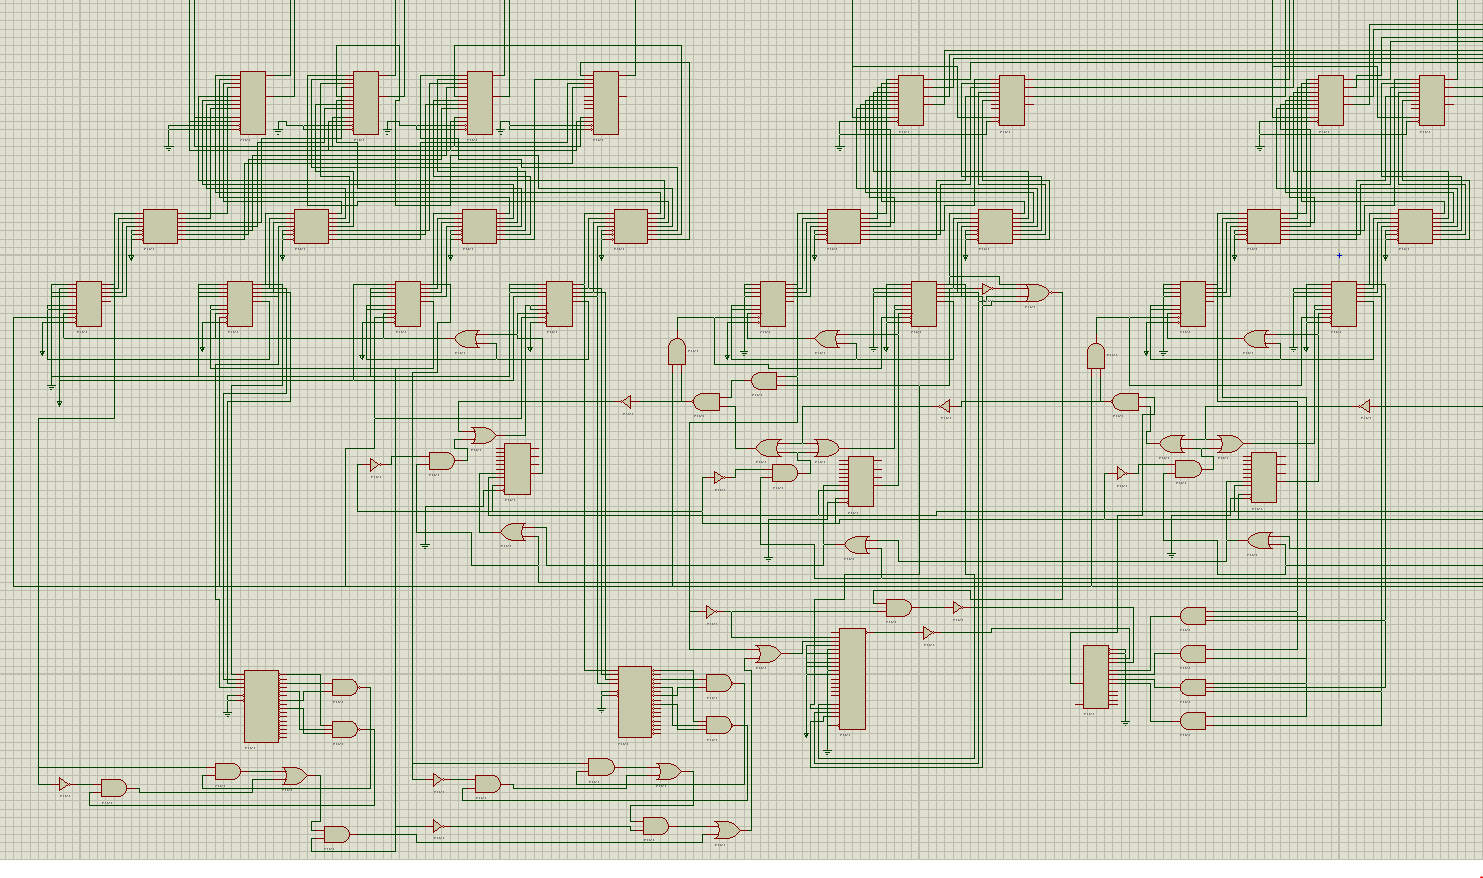
\includegraphics[width=\linewidth]{fig/Counter_4_date.PNG}
\end{figure}
\par 闰年及月份天数选择部分如下
\begin{figure}[H]
    \centering
    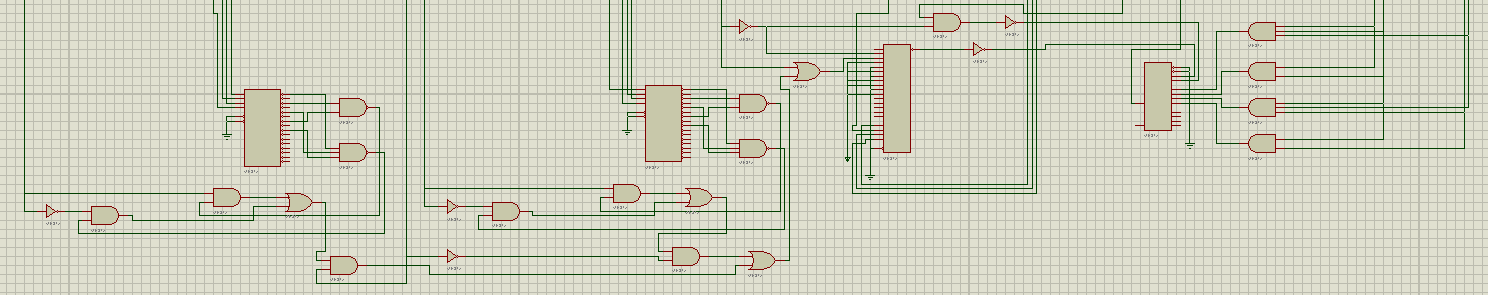
\includegraphics[width=\linewidth]{fig/Counter_4_2.PNG}
\end{figure}
\par 控制端设置如下
\begin{figure}[H]
    \centering
    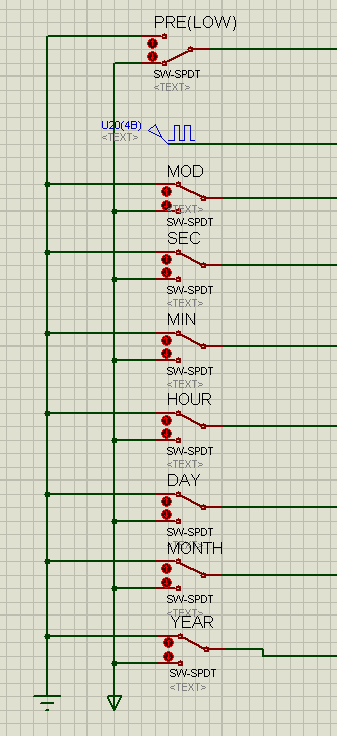
\includegraphics[width=0.3\linewidth]{fig/Counter_3_button.PNG}
\end{figure}


\section{心得体会}
\begin{enumerate}
    \item 本次Proteus仿真的工程量很大,虽然不难,但是需要考虑的细节有很多,既学会了基础十进制计数器的级联及简单模加法器的实现,又学会了大型项目的实施和管理,获益匪浅
    \item 明白时序电路的设计,用Verilog实现了计数器,进一步增强Vivado的使用,不断学习,不断进步
\end{enumerate}


\end{document}